\documentclass{article}
\usepackage[portuguese]{babel}
\usepackage{a4wide}
\usepackage[utf8]{inputenc}
\usepackage{chngpage}
\usepackage{graphicx}
\usepackage{hyperref}
\usepackage{listings}
\usepackage{indentfirst}
\usepackage{float}

\title{Desenvolvimento de Sistemas de Software - Trabalho Prático (Fase Intermédia) - Ano Letivo 2021/2022\\
	\large Grupo 42}
\author{Gonçalo Braz (a93270)
	\and Simão Cunha (a93262)
	\and Tiago Silva (a93277)
	\and Gonçalo Pereira (a93168)}
\date{\today}

\begin{document}
	\begin{minipage}{0.9\linewidth}
        \centering
		\includegraphics[width=0.4\textwidth]{imagens/eng.jpeg}\par\vspace{1cm}
		\href{https://www.uminho.pt/PT}
		{\scshape\LARGE Universidade do Minho} \par
		\vspace{0.6cm}
		\href{https://miei.di.uminho.pt/}
		{\scshape\Large Mestrado Integrado em Engenharia Informática} \par
		\maketitle
		\begin{figure}[H]
		\centering
			\includegraphics[width=3cm, height=3cm]{imagens/braz.png}
			\includegraphics[width=3cm, height=3cm]{imagens/tiago.png}
			\includegraphics[width=3cm, height=3cm]{imagens/simao.png}
			\includegraphics[width=3cm, height=3cm]{imagens/rui.jpg}
		\end{figure}
	\end{minipage}
	
\pagebreak
\tableofcontents
\pagebreak
\maketitle

\section{Prefácio}

Este relatório tem o intuito de apresentar a fase intermédia do trabalho prático proposto na UC de \textit{Desenvolvimento de Sistemas de Software}: implementar um sistema de gestão para centros de reparação de equipamentos eletrónicos. \par

Nesta fase, serão apresentados dois modelos: o \textbf{Modelo de domínio} (com as identidades relevantes) e o \textbf{Modelo de Use Case} (diagramas + especificações do \textit{Use Case} com as funcionalidades propostas). \par

O \textbf{Modelo de domínio} captura as entidades dos problemas e os relacionamentos entre elas. É a base da análise de requisitos, uma vez que fornece uma \textit{framework} concetual para raciocinar sobre o problema.

O \textbf{Modelo de Use Case} descreve como os atores atingem certos objetivos utilizando o sistema, explicitando eventuais comportamentos alternativos ou exceções.

Como pontapé de saída, a equipa docente disponibilizou alguns cenários de utilização dos serviços do centro de reparação para a análise de requisitos, com vista à elaboração do modelo de domínio e do modelo de \textit{Use Case}.


\section{Descrição do trabalho realizado}
O sistema proposto deve ser capaz de gerir os pedidos de reparação de equipamentos que cheguem ao centro, assim como as respetivas respostas dos técnicos e dos gestores. \par
Para tal, utilizamos a linguagem UML para elaborar o modelo de domínio que demonstra todas as
interações que decorrem no sistema que pretendemos implementar e para elaborar o modelo de \textit{use case} que irá associar cada ator ao seu \textit{use case} - interações com o sistema que satisfazem cenários propostos.

\subsection{Modelo de Domínio}
Depois de analisar os cenários dados pela equipa docente no enunciado do trabalho prático, foi
feito um estudo acerca dos conceitos que melhor representariam o sistema a implementar. \par

\begin{table}[H]
\centering
\scalebox{1}{
\begin{tabular}{|c|}
\hline
\textbf{Entidades do sistema} \\ \hline
Cliente                       \\ \hline
Pedido                        \\ \hline
Equipamento                   \\ \hline
Funcionário                   \\ \hline
Gestor                        \\ \hline
Técnico                       \\ \hline
Custo                         \\ \hline
\end{tabular}
}
\end{table}
 De seguida, passamos à tradução das suas relações de modo a serem identificáveis no modelo do domínio.
 \par Começando pelo componente-raíz deste trabalho, o \textit{Pedido de arranjo de um Equipamento}. Este é realizado por um \textbf{Cliente} e será atendido por um \textbf{Funcionário} da loja.
 \par O \textbf{Pedido} terá um custo que poderá ser fixo, no caso dele se tratar de um pedido associado a um disponível \textit{Serviço Expresso}, ou então poderá ter um custo que dependerá do decorrer da reparação do sujeito do pedido.
 \par O \textbf{Funcionário} é um Utilizador do sistema que este trabalho descreve, estando incluido dentro deste numa \textit{Lista de Funcionários}. A sua função consiste na interação com o \textbf{Cliente}.
 \par Entre os outros utilizadores constam os \textbf{Técnico}'s e o \textbf{Gestor}, estando os técnicos incluídos numa lista própria tal como a entidade anteriormente referida.
 \par O \textbf{Gestor} é a entidade com autorização máxima dentro do sistema, sendo o único capaz de consultar e editar as listas mencionadas.
 \par O \textbf{Técnico} é a entidade responsável pela resolução das requisições dos clientes, sendo este que mediante o decorrer da reparação atualiza o estado do custo no sistema de modo a este verificar se o mesmo não ultrapassa o \textit{Orçamento} descrito ao \textbf{Cliente}. O \textbf{Pedido} a ser resolvido é retirado da \textit{Lista de Pedidos de Reparação}, preferencialmente tratando o caso mais antigo ou mais urgente (no caso da existência de um \textit{Serviço Expresso} em vias de expirar),
 \par O \textbf{Cliente} é identificado pelo seu \textit{NIF} e pode ser contactado através do seu \textit{Email} ou \textit{Telemóvel}.
 
\begin{figure}[H]
    \centering
    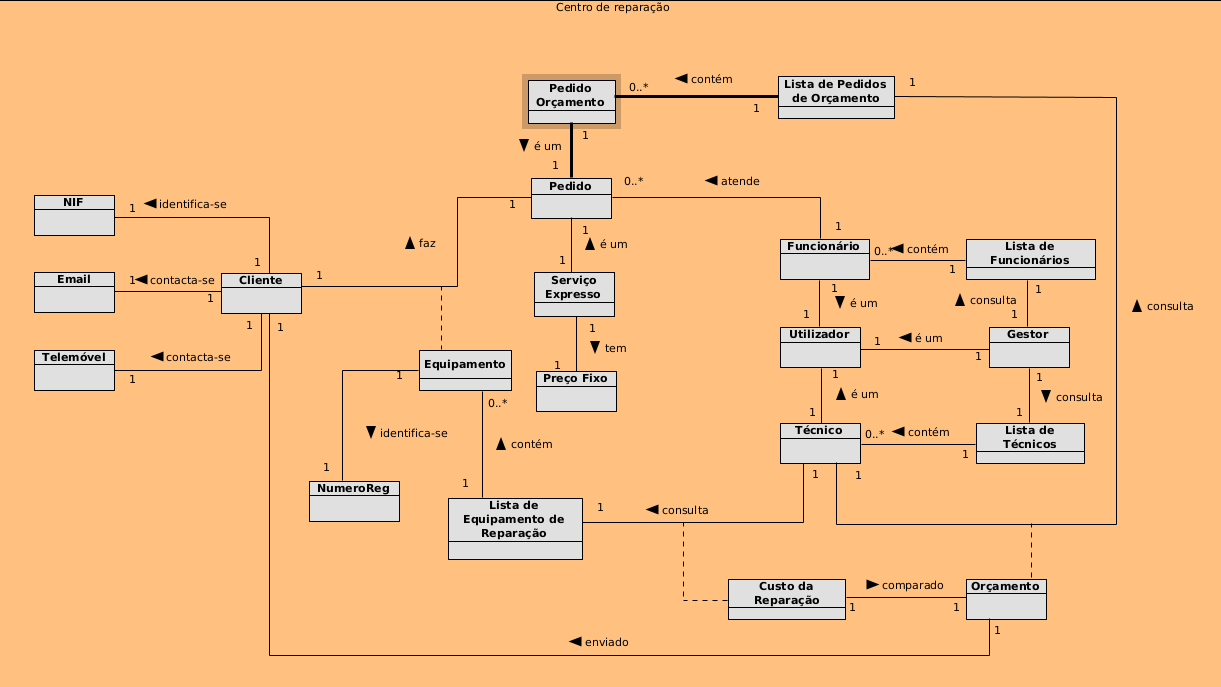
\includegraphics[width=\textwidth]{imagens/modeloDominio.png}
    \caption{Modelo de Domínio}
\end{figure}

\subsection{Modelo de \textit{Use Case}}

Terminado o estudo do modelo de Domínio, iniciamos a dissecação do modelo de \textit{Use Case}.
\par Começamos por identificar os atores do sistema. Para o nosso problema, reconhecemos que estes serão o \textbf{Funcionário}, \textbf{Gestor} e \textbf{Técnico}.
\par As utilizadores têm como primeira opção - essencial para desbloquear todas as outras - a sua autenticação no sistema.
\par Após este passo um \textbf{Técnico} é capaz de criar um orçamento ou de processar uma reparação.
\par No caso do \textbf{Funcionário}, ele conseguirá registar um \textit{pedido de orçamento}, um \textit{pedido de serviço expresso}, a \textit{entrega de um orçamento}, e a\textit{ resposta de um cliente} sobre o orçamento correspondente a um seu pedido.
\par Como administrador, o \textbf{Gestor} tem poder para, além de realizar todas as operações que os outros dois cargos, é capaz de aceder às listas: de todos os técnicos, de todos os funcionários, e do exaustivo \textit{log} de todas as intervenções de um técnico. 

\begin{table}[H]
\centering
\resizebox{15.5cm}{1.2cm}{%
\begin{tabular}{ccc}
\hline
\multicolumn{3}{c|}{\textbf{Entidades do sistema}}                                                                                                                           \\ \hline
\multicolumn{1}{c|}{\textbf{Funcionário}}                                      & \multicolumn{1}{c|}{\textbf{Gestor}}                   & \textbf{Técnico}                                     \\ \hline
\multicolumn{1}{c|}{Autenticar-se no sistema}                         & \multicolumn{1}{c|}{Autenticar-se no sistema} & Autenticar-se no sistema                    \\ \hline
\multicolumn{1}{c|}{Registar pedido de orçamento}                     & \multicolumn{1}{c|}{Criar orçamento}          & Aceder à listagem com stats de cada técnico \\ \hline
\multicolumn{1}{c|}{Registar entrega do equipamento} &
\multicolumn{1}{c|}{Processamento de reparação} & Aceder à listagem com stats dos funcionários \\ \hline
\multicolumn{1}{c|}{Registar pedido do serviço expresso} & \multicolumn{1}{c|}{Registar novo cliente} & \multicolumn{1}{c}{Aceder à listagem exaustiva para cada técnico de todas as intervenções} \\ \cline{1-2}
\multicolumn{1}{c|}{Registar a resposta do cliente sobre o orçamento} & \multicolumn{1}{c|}{Registar novo utilizador}                                              \\ \hline
\end{tabular}
}
\caption{Entidades do sistema com os respetivos \textit{Use Case}}
\end{table}




Assim, desenhamos quatro diagramas de \textit{Use Case}: 

\par Iniciamos com o caso geral do sistema, com as funcionalidades principais de cada um dos atores que interagem com o mesmo. 
\par O \textbf{Funcionário} tem como principal função adicionar registos no sistema, tal como novos pedidos ou respostas dadas pelos clientes.
\par O \textbf{Técnico} é responsável por processar reparações e anunciar o decorrer das mesmas assim como a soma do custo no momento.
\par O \textbf{Gestor}, consegue realizar todas as funções dos outros dois atores e adicionalmente, é capaz de concretizar consultas no sistema que não estão disponíveis para os outros, tais como aceder à lista dos funcionários ou dos técnicos.
\par Todas estas funções têm como inferido a pré autenticação destes utilizadores no sistema.

\begin{figure}[H]
    \centering
    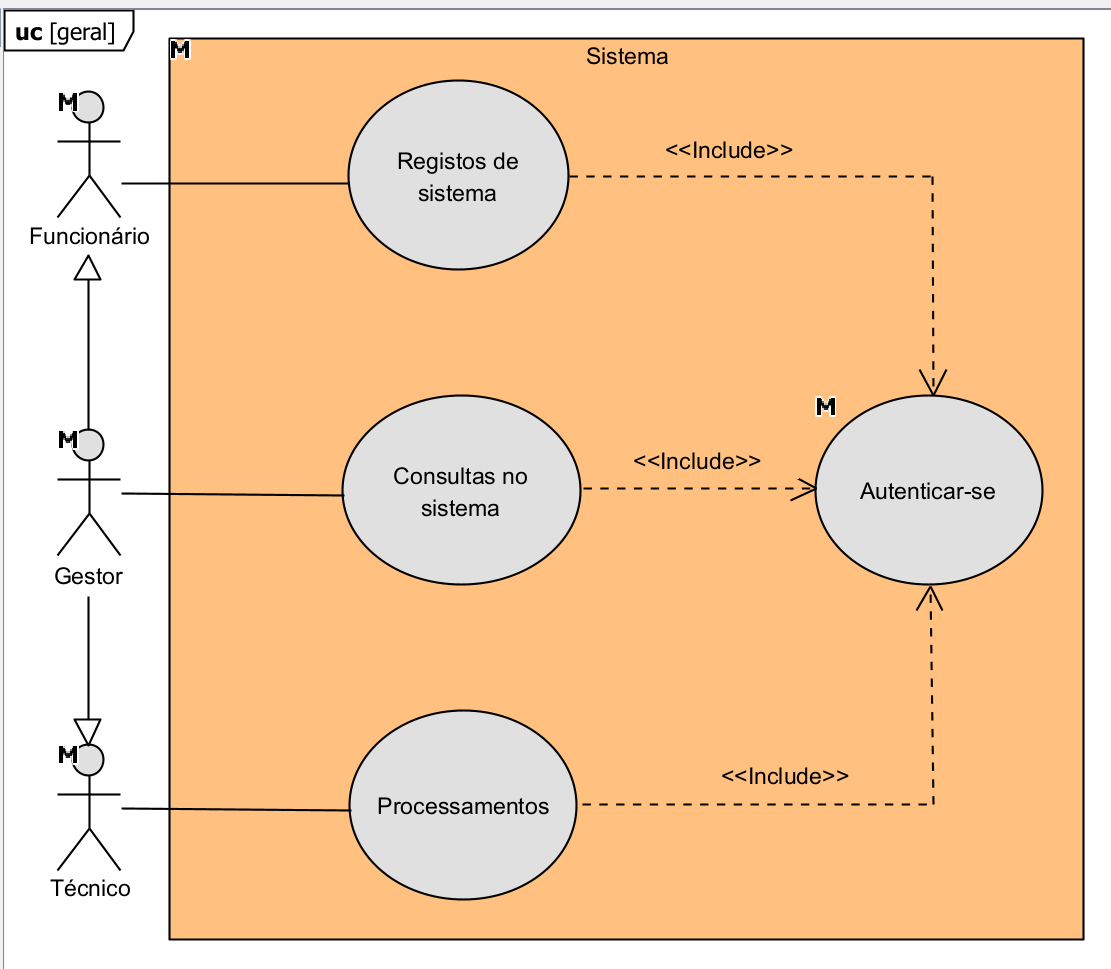
\includegraphics[width=\textwidth]{imagens/ucGeral.png}
    \caption{Modelo geral de \textit{Use Case}}
\end{figure}

\par Seguimos com um olhar mais detalhado sobre a efetuação de registos no sistema que, reiterando, são apenas realizados pelo \textbf{Funcionário} e pelo \textbf{Gestor}.
\par O \textbf{Funcionário} é portanto capaz de registar um novo cliente, um pedido de orçamento, um pedido de serviço expresso e a entrega de um equipamento, que por sua vez o sistema interpretará de forma a atualizar os seus dados de acordo.
\par No caso do \textbf{Gestor}, este extende o anterior, sendo adicionalmente capaz de registar um novo \textbf{Técnico} ou \textbf{Funcionário}.

\begin{figure}[H]
    \centering
    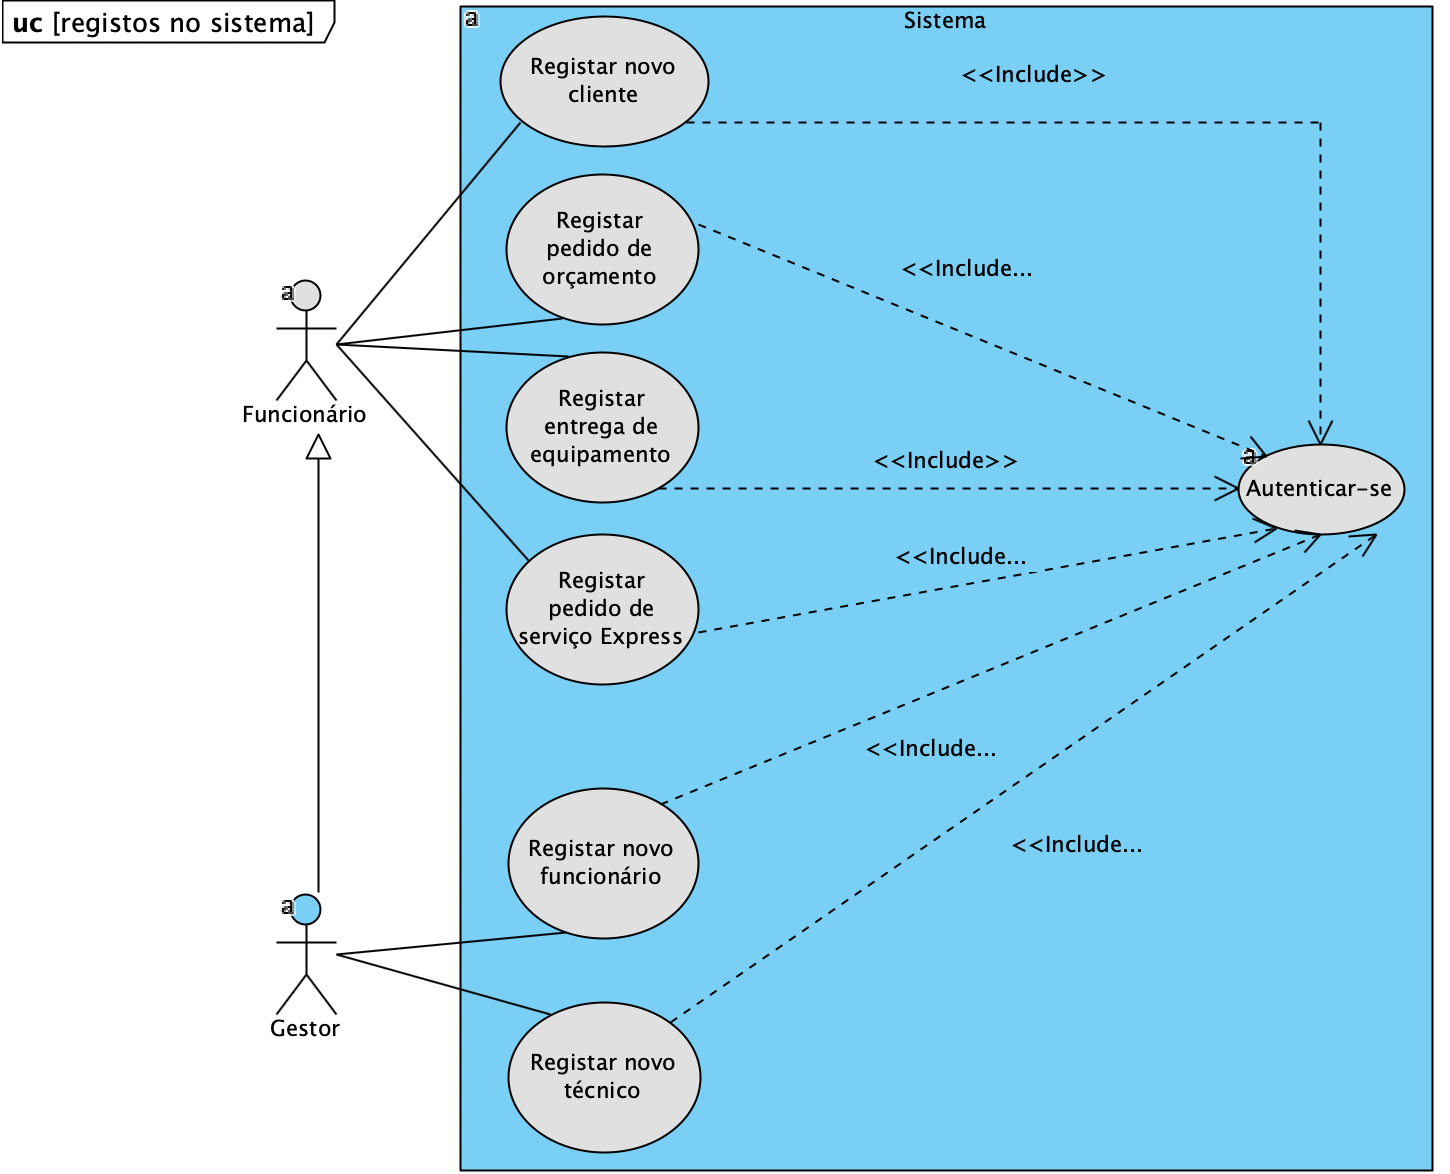
\includegraphics[width=\textwidth]{imagens/usecaseRegistos.png}
    \caption{Modelo \textit{Use Case} dos registos no sistema}
\end{figure}

\par O \textbf{Técnico} é capaz de processar a reparação e de criar um orçamento. 
\par Tal como nos casos anterirores, o \textbf{Gestor} apresenta as mesmas possibilidades do técnico.

\begin{figure}[H]
    \centering
    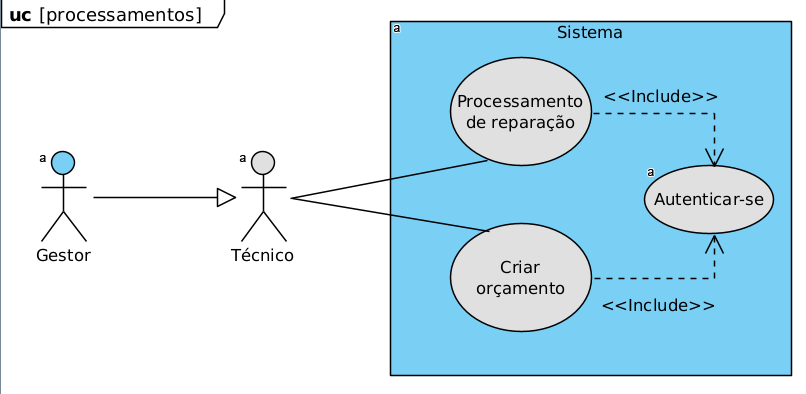
\includegraphics[width=\textwidth]{imagens/useCaseProcessamento.png}
    \caption{Modelo \textit{Use Case} do processamento}
\end{figure}

\par Os \textit{Use Cases} únicos ao \textbf{Gestor} são as opções de consulta das listagens dos funcionários, técnicos e das intervenções destes últimos. 

\begin{figure}[H]
    \centering
    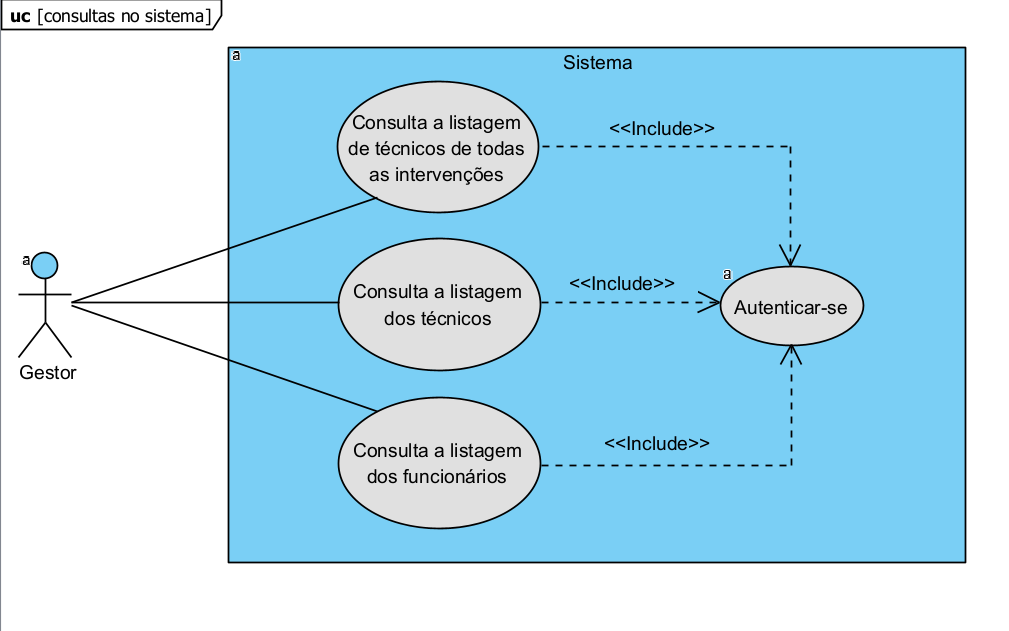
\includegraphics[width=\textwidth]{imagens/ucConsultas.png}
    \caption{Modelo \textit{Use Case} das consultas no sistema}
\end{figure}


\pagebreak


\section{Descrição dos \textit{Use Cases}}

\begin{figure}[H]
    \centering
    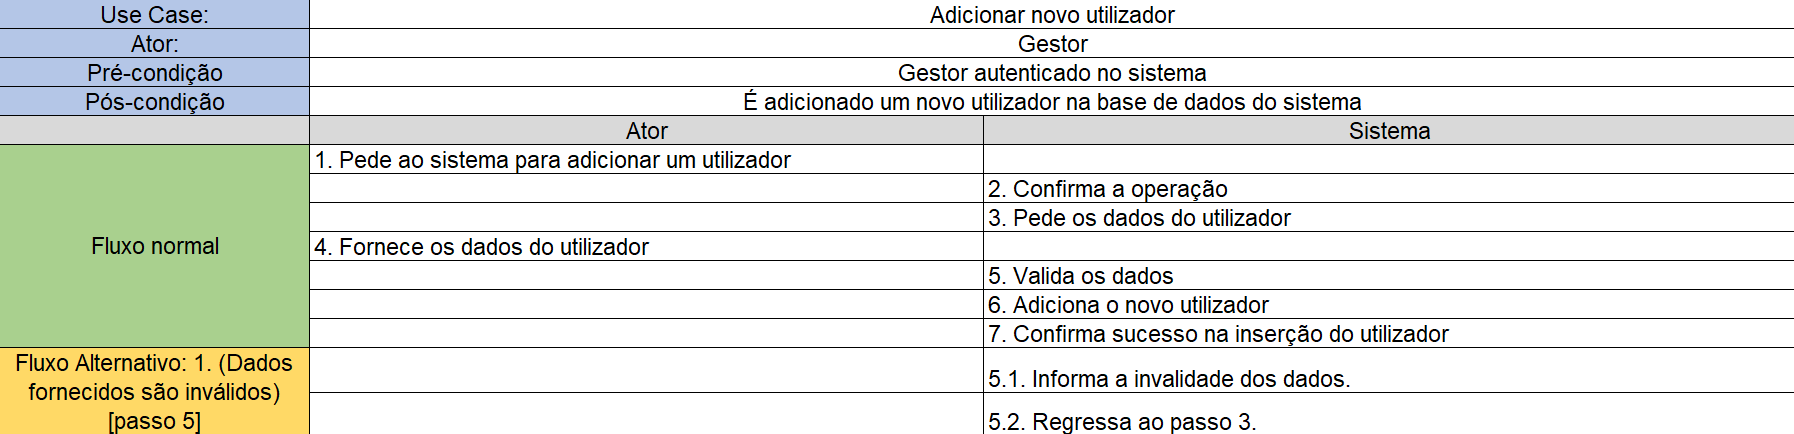
\includegraphics[width=\textwidth]{imagens/adicionar_utilizador.png}
    \caption{\textit{Use Case} da adição de um novo utilizador}
\end{figure}

\begin{figure}[H]
    \centering
    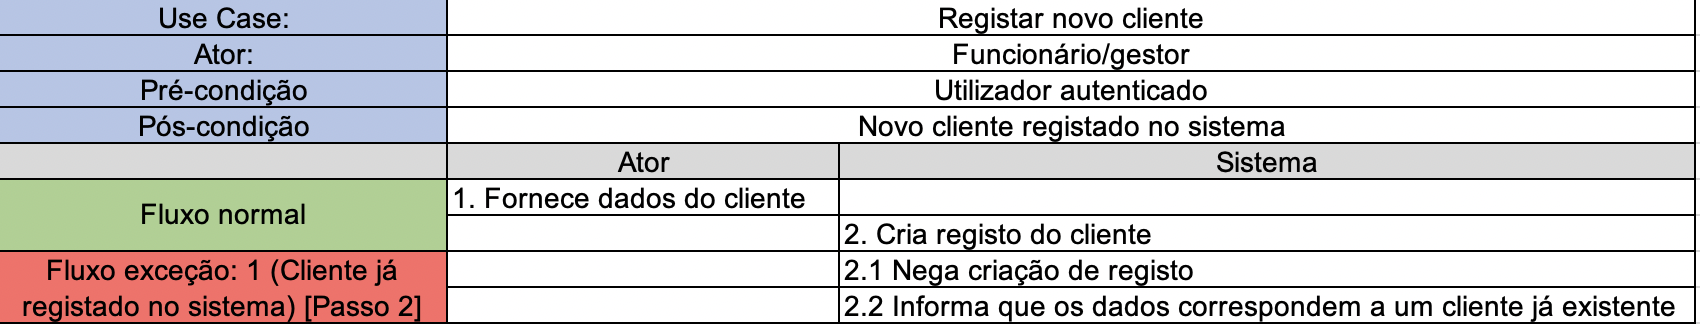
\includegraphics[width=\textwidth]{imagens/registar_novo_cliente.png}
    \caption{\textit{Use Case} do registo de um novo cliente}
\end{figure}

\begin{figure}[H]
    \centering
    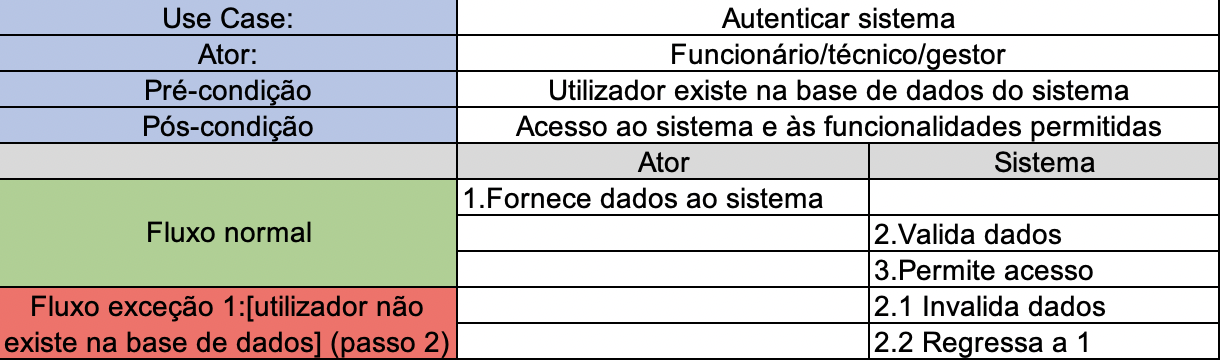
\includegraphics[width=\textwidth]{imagens/autenticar_sistema.png}
    \caption{\textit{Use Case} da autenticação no sistema}
\end{figure}

\begin{figure}[H]
    \centering
    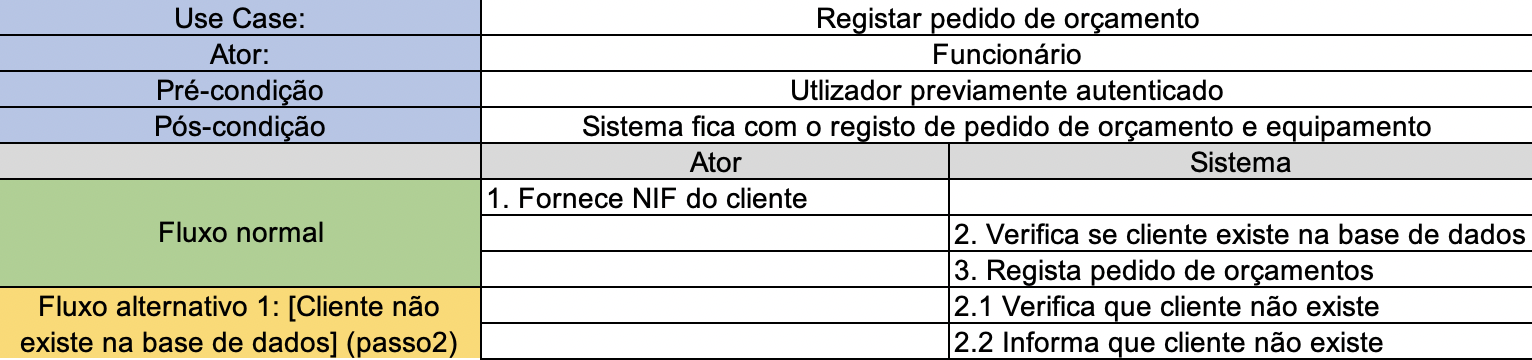
\includegraphics[width=\textwidth]{imagens/registarPedidoOrcamento.png}
    \caption{\textit{Use Case} do registo de pedido de orçamento}
\end{figure}

\begin{figure}[H]
    \centering
    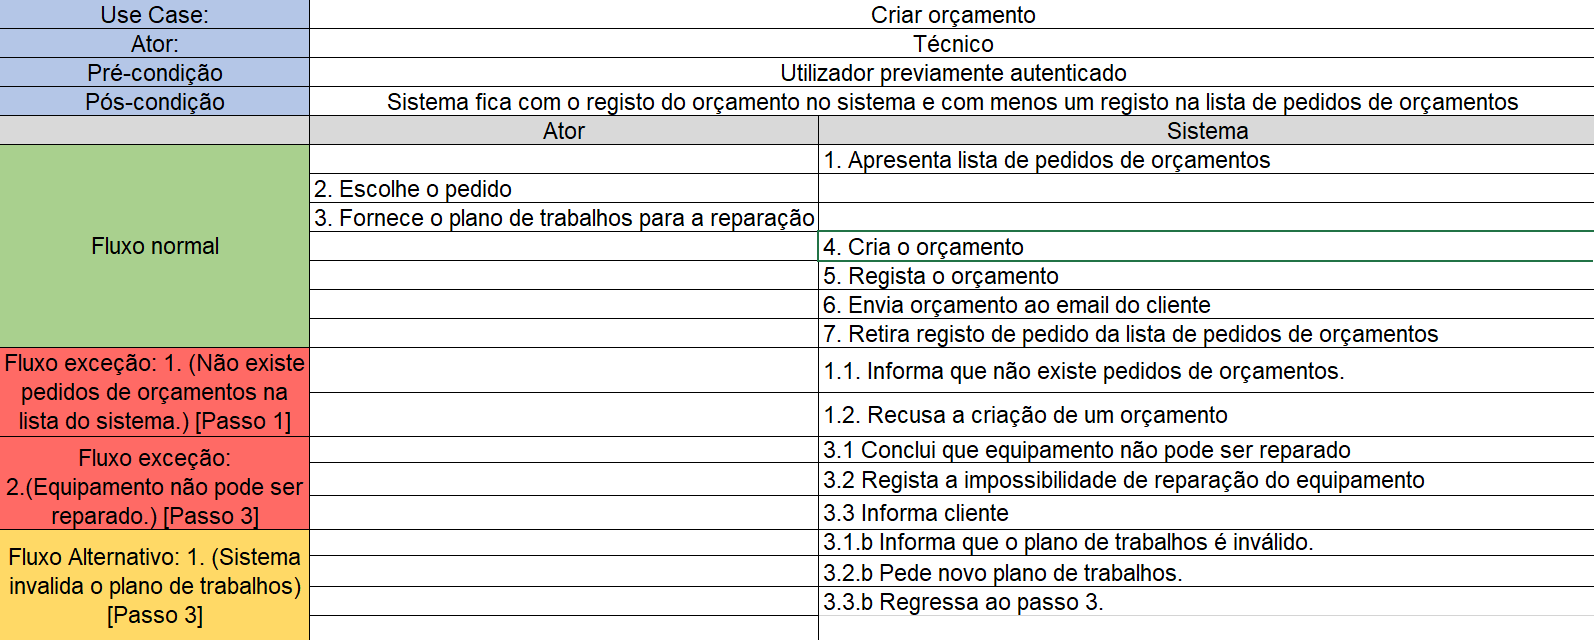
\includegraphics[width=\textwidth]{imagens/criar_orcamento.png}
    \caption{\textit{Use Case} do registo da criação do orçamento}
\end{figure}

\begin{figure}[H]
    \centering
    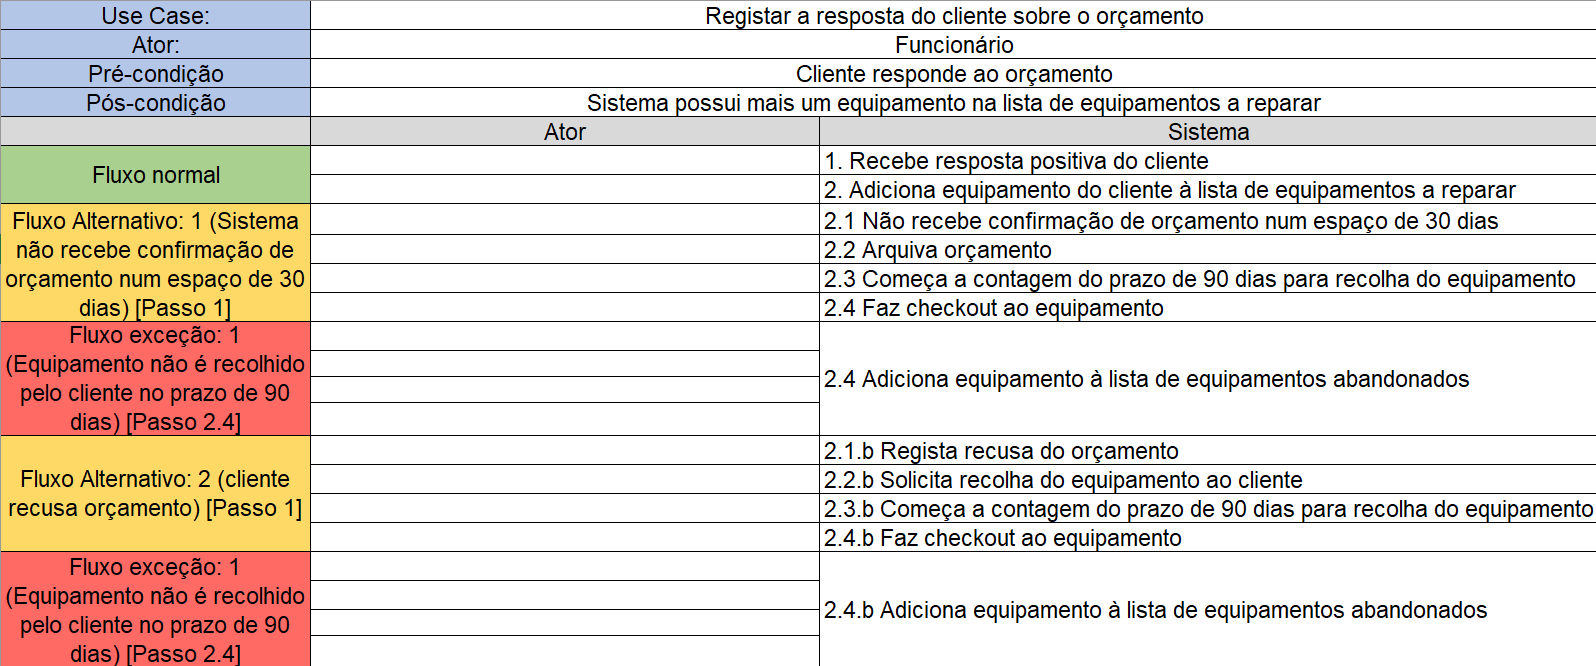
\includegraphics[width=\textwidth]{imagens/registar_resposta_cliente_orcamento.png}
    \caption{\textit{Use Case} da resposta do cliente ao orçamento}
\end{figure}

\begin{figure}[H]
    \centering
    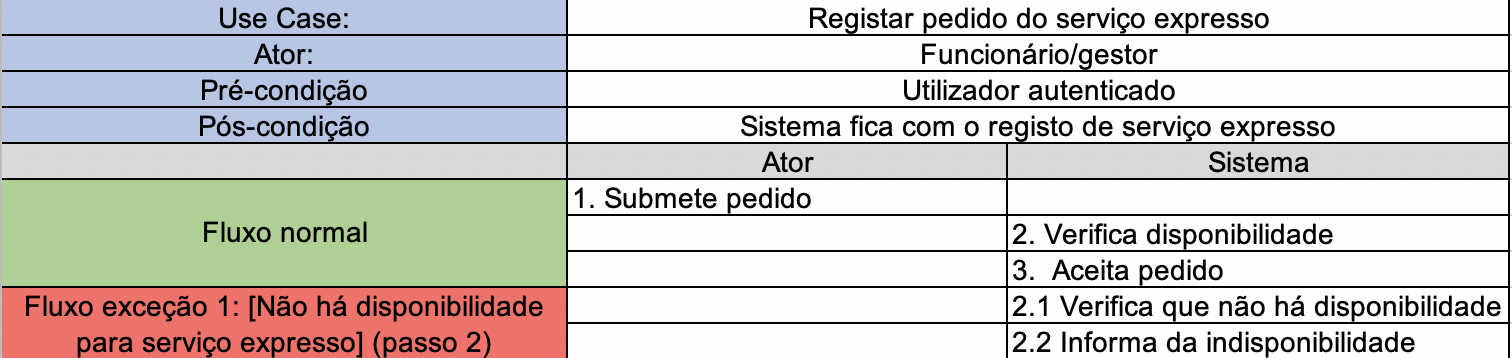
\includegraphics[width=\textwidth]{imagens/registarServicoExp.png}
    \caption{\textit{Use Case} do registo do serviço}
\end{figure}

\begin{figure}[H]
    \centering
    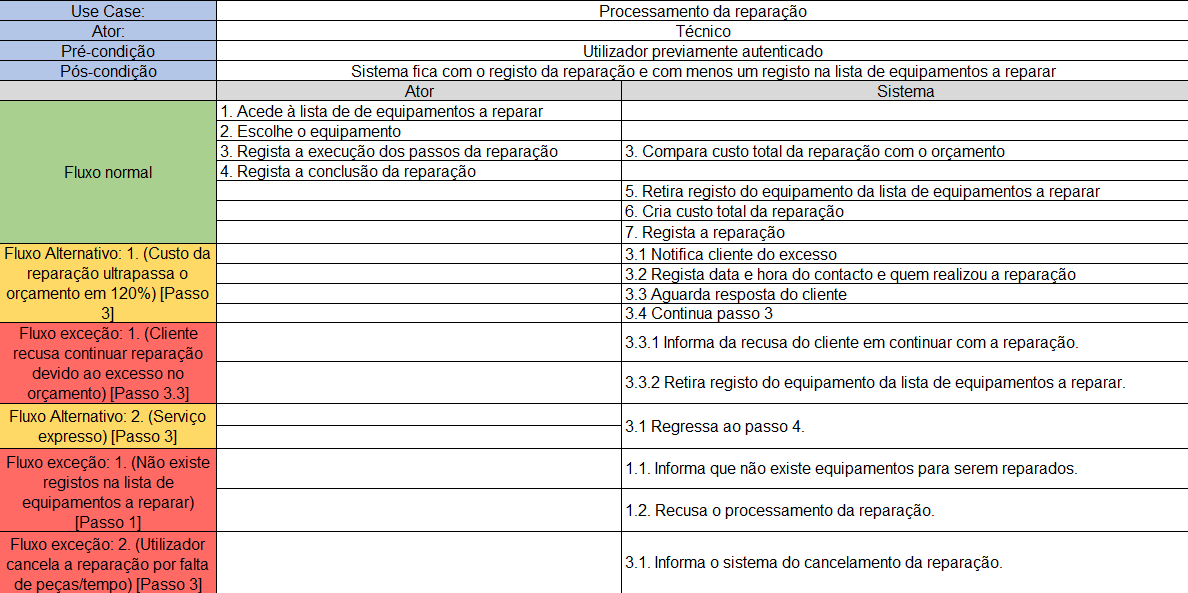
\includegraphics[width=\textwidth]{imagens/processamento_reparacao.png}
    \caption{\textit{Use Case} do processamento da reparação do equipamento}
\end{figure}

\begin{figure}[H]
    \centering
    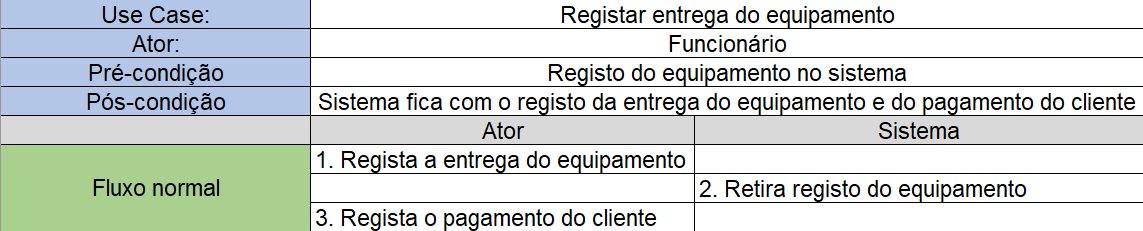
\includegraphics[width=\textwidth]{imagens/registar_entrega_equipamento.png}
    \caption{\textit{Use Case} da entrega do equipamento}
\end{figure}

\begin{figure}[H]
    \centering
    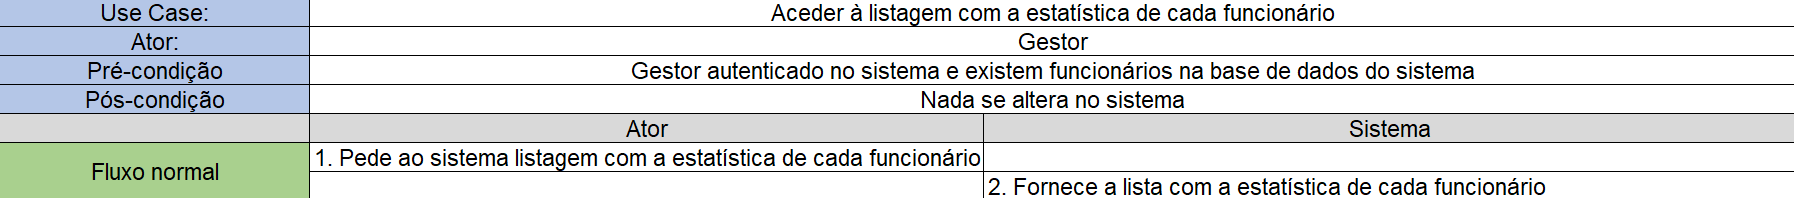
\includegraphics[width=\textwidth]{imagens/aceder_lista_funcionarios.png}
    \caption{\textit{Use Case} do acesso à lista dos funcionários}
\end{figure}

\begin{figure}[H]
    \centering
    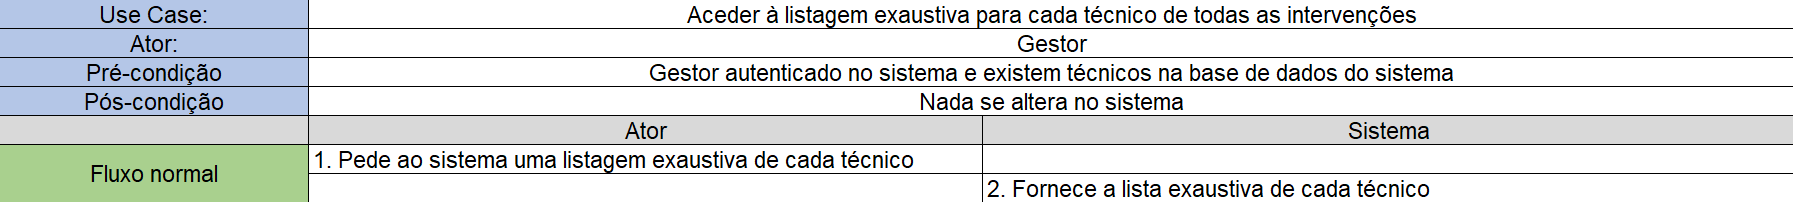
\includegraphics[width=\textwidth]{imagens/aceder_lista_tecnicos.png}
    \caption{\textit{Use Case} do acesso à lista dos técnicos}
\end{figure}

\section{Conclusão}

\par Para esta primeira fase do projeto acreditamos ter desenvolvido uma base sólida e fundamental para a construção do software no futuro.
\par Conseguimos perceber que planear e modelar previamente uma aplicação é tão importante como a escrita do seu código. Sem este trabalho, haveria certamente a necessidade de refazer a nossa aplicação várias vezes, levando a um desenvolvimento mais demorado e ineficaz.
\par Assim, o \textit{modelo de domínio} foi concluído de forma a ser esclarecedor e ao mesmo tempo conciso, permitindo uma legibilidade adequada das relações entre as entidades do projeto mesmo por entidades que não estejam inteiramente a par da tecnicidade de construção de \textit{software}. 
\par A formulação dos \textit{casos de uso} favoreceu a deteção de incongruências no \textit{modelo de domínio}. Além disso, o modelo de \textit{Use Case} sintetiza de forma clara as várias operações que o sistema permitirá serem realizadas, assim facilitando uma planificação do trabalho futuro. 

\end{document}
